\documentclass[10pt,conference,a4paper]{IEEEtran}

% ----- Packages -------------------------------------------------------------
\usepackage{cite}
\usepackage{amsmath,amssymb,amsfonts}
\usepackage{algorithmic}
\usepackage{graphicx}
\usepackage{booktabs}
\usepackage{textcomp}
\usepackage{xcolor}
\usepackage[hidelinks]{hyperref}
\usepackage[capitalise]{cleveref}
\usepackage{caption}
\usepackage{cuted}
\captionsetup{font=small,labelfont=bf}

\graphicspath{{../assets/2026-05-20_principled_ml_calib/}}

\renewcommand{\arraystretch}{1.15}

\newcommand{\Suv}{\Delta\mathbf{uv}}
\newcommand{\W}{\mathbf{W}}
\newcommand{\Sig}{\boldsymbol{\Sigma}}
\newcommand{\R}{\mathbb{R}}
\newcommand{\Lnll}{\mathcal{L}_{\mathrm{NLL}}}

% ============================================================================
\begin{document}

\title{Principled ML for LiDAR--Camera Calibration:\\
       a Per-Point Trust Head Supervised Through a Closed-Form Solver}

\author{\IEEEauthorblockN{Hiroyuki Funaya}
\IEEEauthorblockA{Toyota Research --- Advanced Development\\
hiroyuki.funaya@example.com}}

\maketitle

% ----- Hero figure (full-width, immediately under the title) ----------------
\begin{strip}
\centering
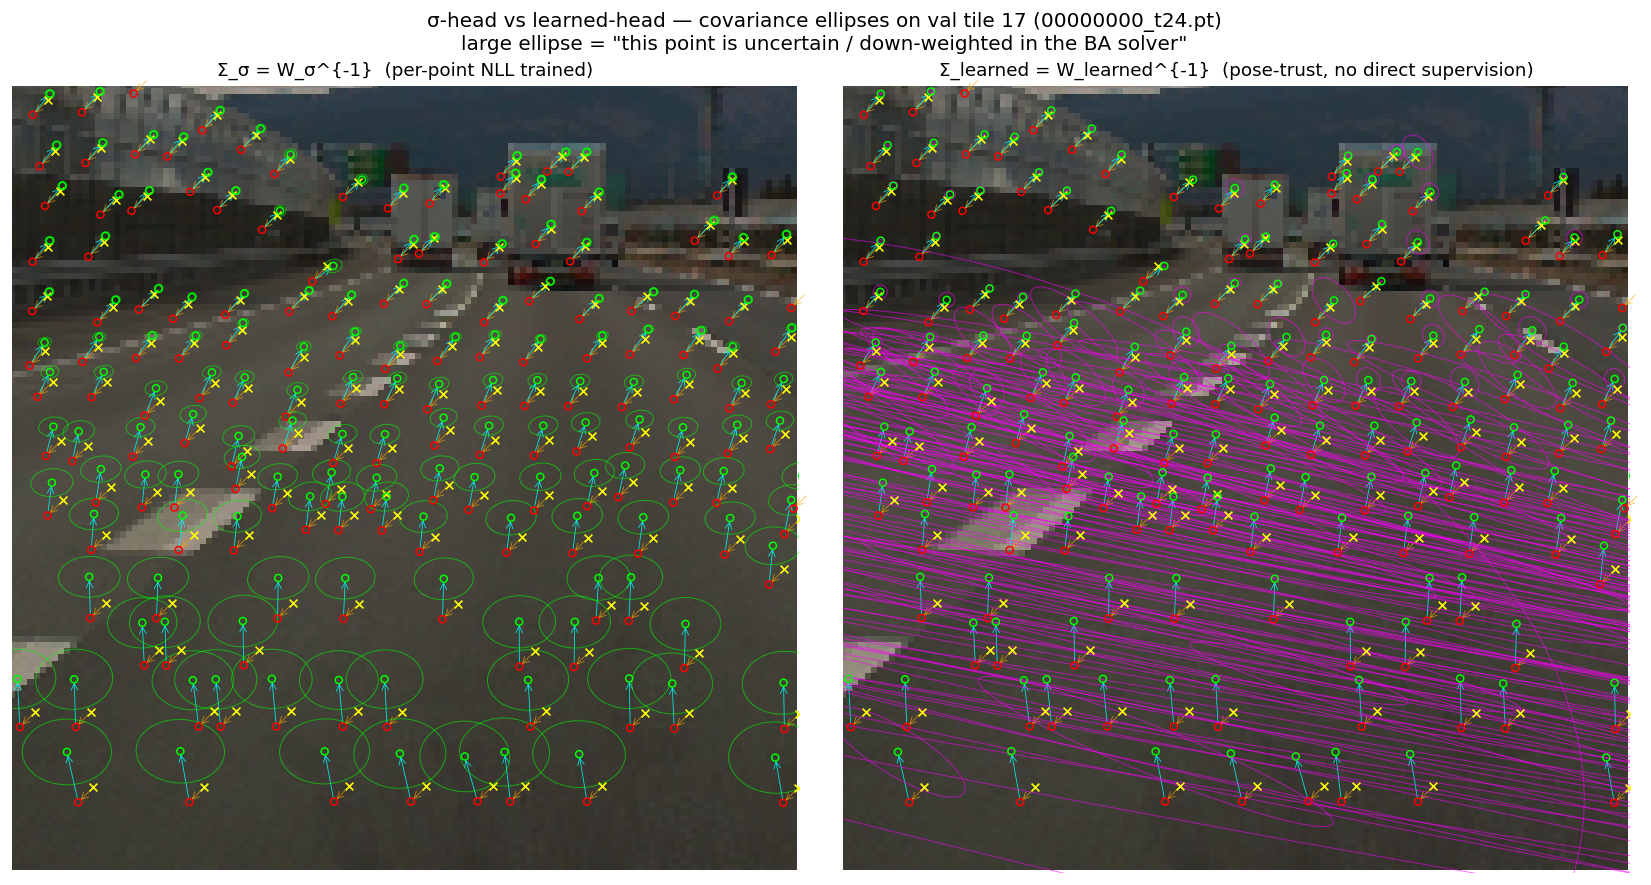
\includegraphics[width=0.96\linewidth]{sigma_compare_idx17.png}
\captionof{figure}{\textbf{$\sigma$-head (left) vs.\ learned head
(right) on the same val tile.} Same frozen backbone, same per-query
feature $\mathbf{q}_i$. Ellipses are $\Sig_i = \W_i^{-1}$.
\textbf{Left}: the existing per-point head trained with Gaussian NLL on
the optical-flow residual $\Suv$. Ellipses are uniformly small,
including on the road, because $\Suv$ is locally consistent on asphalt.
\textbf{Right}: a new $\sim$100\,k-param head trained \emph{only}
through a closed-form Gauss--Newton pose solver, with no direct loss on
$\W$. The road is suppressed (large ellipses = ``don't trust me for
pose''), and on the road the ellipses are elongated horizontally---the
network discovered on its own that a road-plane point sliding along the
surface is uninformative about yaw, a structural property of the
inverse problem that a scalar-confidence head provably cannot
represent.}
\label{fig:hero}
\bigskip

\captionof{table}{\textbf{Phases 1, 1.b, and 1.c on a single page.}
Held-out $\delta$-MSE (deg$^2$) and per-axis RMSE on
$(\omega_x,\omega_y)\le 0.3^\circ$ perturbations. Same frozen backbone,
same loss, same MLP head architecture across phases. \textbf{Phase 1}:
single tile (idx 17), train$\equiv$eval on $N{=}100$ perturbations
(sign-of-life only). \textbf{Phase 1.b}: same single tile, fresh
$(\omega_x,\omega_y)$ each step ($B{=}16$, 400 steps), held-out
$N{=}200$ perturbations on the same tile---the head must generalise
across pose draws but not across scenes. \textbf{Phase 1.c}: same
recipe but the train stream samples a fresh \emph{(KAMIKADO train
tile, perturbation)} pair at each step ($B{=}16$, 400 steps over 27\,880
training tiles) and the held-out batch is $N{=}512$ random
\emph{val} tiles, each with one fresh perturbation---the head must
generalise across both pose draws \emph{and} scenes. The degenerate
single-tile column (last) re-runs Phase~1.b on a near-featureless
asphalt+fence tile (idx 0) as a sanity check.}
\label{tab:combined}
\begin{tabular}{lcccccc}
\toprule
                       & \multicolumn{1}{c}{\textbf{Phase 1}}
                       & \multicolumn{2}{c}{\textbf{Phase 1.b}}
                       & \multicolumn{2}{c}{\textbf{Phase 1.c (multi-tile)}}
                       & \multicolumn{1}{c}{\textbf{Degenerate}} \\
\cmidrule(lr){2-2}\cmidrule(lr){3-4}\cmidrule(lr){5-6}\cmidrule(lr){7-7}
$\W$ source            & $\delta$-MSE
                       & $\delta$-MSE     & RMSE/axis
                       & $\delta$-MSE     & RMSE/axis
                       & $\delta$-MSE \\
                       & \footnotesize{(train$\equiv$eval, N=100)}
                       & \footnotesize{(idx17, N=200)} & \footnotesize{(idx17)}
                       & \footnotesize{(KAMIKADO val, N=512)} & \footnotesize{(KAMIKADO val)}
                       & \footnotesize{(idx 0, N=200)} \\
\midrule
do-nothing $(\delta=0)$         & ---               & $0.030$           & $0.18^\circ$           & $0.0253$          & $0.16^\circ$           & $0.030$ \\
$\W = I$ (uniform)              & $0.111$           & $0.0458$          & $0.21^\circ$           & $0.1741$          & $0.42^\circ$           & $0.137$ \\
$\W = \sigma$-head (NLL)        & $0.106$           & $0.0146$          & $0.12^\circ$           & $0.1503$          & $0.39^\circ$           & $0.132$ \\
$\W = $ \textbf{learned (ours)} & $\mathbf{0.0107}$ & $\mathbf{0.0066}$ & $\mathbf{0.081^\circ}$ & $\mathbf{0.0978}$ & $\mathbf{0.31^\circ}$  & $\mathbf{0.0254}$ \\
\bottomrule
\end{tabular}
\end{strip}

% ----- Abstract --------------------------------------------------------------
\begin{abstract}
We propose a calibration network whose output is not a 6-DoF pose but a
per-point information matrix $\W_i \in \R^{2\times 2}$. The pose is
recovered by a closed-form Gauss--Newton (GN) step that consumes the
network's outputs together with the camera intrinsics and per-point
geometry. The information head is supervised \emph{exclusively} by the
gradient of the pose loss flowing back through the GN solver---there is
no direct loss on $\W$.
On a typical highway tile (Phase 1.b) the learned head reaches
$\delta$-MSE $0.0066\;\mathrm{deg}^2$ on held-out perturbations,
$2.2\times$ better than the existing per-point $\sigma$-head ($0.0146$)
and $7\times$ better than uniform weighting ($0.046$). When the
\emph{same head} is trained across the entire KAMIKADO training split
and evaluated on a held-out batch of $N{=}512$ val tiles (Phase 1.c),
it reaches $0.098\;\mathrm{deg}^2$ versus $0.150$ for the $\sigma$-head
and $0.174$ for uniform---$1.5\times$ over the $\sigma$-head; both
$\sigma$-head and uniform are now \emph{worse than predicting
$\delta{=}0$} across the multi-tile val set, which is precisely the
NLL-vs-pose-trust failure mode the design predicts.
All numbers come from a $\sim$100\,k-parameter MLP added on top of a
\emph{frozen} backbone. The learned $\W$ field reproduces, without
prompting, the classical photogrammetric ``sliding null-space'' of road
planes: ellipses on the road are large \emph{and elongated horizontally}
in the yaw direction, a structural property a scalar-confidence head
cannot express.
\end{abstract}

% ----- 1. Introduction --------------------------------------------------------
\section{Introduction}

The previous baseline~\cite{cite:CalibNetDepth} outputs, per LiDAR
query, a flow correction $\Suv$ together with a $2{\times}2$ residual
covariance $\Sig$, supervised by negative log-likelihood
%
\begin{equation}
\Lnll = \tfrac{1}{2}\,\mathbf{r}^\top \Sig^{-1}\mathbf{r}
        + \tfrac{1}{2}\log\det\Sig,
\quad
\mathbf{r} = \Suv - \Suv_{gt}.
\label{eq:nll}
\end{equation}
%
This trains $\Sig$ to reflect \emph{the variance of per-point flow
residuals}, \emph{not} how much the point should be trusted when
recovering a pose. The two are not the same. A road tile's flow is
locally consistent (so per-point NLL learns small $\Sig$ there), yet
the road is precisely the worst input to a pose estimator: a thousand
nearly co-planar points pin yaw and pitch to the ground plane rather
than to the scene, and any coherent flow error on the road propagates
into pose with full weight. Existing systems patch over this with
heuristics such as $\sigma$-stratified top-$K$ sampling.

\textbf{Contribution.} We argue that the right place to supervise
``trust'' is \emph{through the pose solver}, not via a per-point
auxiliary loss. Concretely, we keep the existing image/LiDAR
cross-attention backbone frozen, and add a small head
$\mathrm{InfoHead2x2}: \mathbf{q}_i \mapsto \W_i = L_iL_i^\top + \epsilon I$
that produces a $2{\times}2$ information matrix per query. A
closed-form 2-DoF GN step consumes $(\Suv_i, \W_i, z_i, K)$ and emits
the calibration delta $\delta$. The head is supervised only by
$\|\delta - \delta_{gt}\|^2$. We show on a held-out batch of
perturbations that the learned $\W$ field beats the existing
$\sigma$-head by $2.2\times$, beats uniform weighting by $7\times$,
and recovers structural properties of the inverse problem (road
suppression, on-road yaw-direction anisotropy) that a scalar-confidence
head provably cannot represent.

% ----- 2. Related work --------------------------------------------------------
\section{Related work}

\textbf{Differentiable solvers in the loop.}
DROID-SLAM~\cite{teed2021droid} is the closest piece of prior art in
spirit: dense optical flow plus a per-pixel \emph{confidence map}, fed
into a differentiable bundle adjustment that solves for trajectory and
depth. The confidence is supervised exclusively through the BA layer,
exactly the trick we use for $\W$. We solve a different and smaller
problem (a few-DoF calibration delta from a single LiDAR-camera
frame) and predict $2{\times}2$ matrices rather than per-pixel
scalars, which is what enables the on-road yaw anisotropy
of~\cref{sec:phase1b}.

\textbf{Differentiable optimisation as a layer.}
OptNet~\cite{amos2017optnet} and the broader declarative-network
literature~\cite{gould2021deep} establish that one can backpropagate
through the solution of an inner optimisation problem via the
implicit-function theorem. Our pose update
$\delta = (J^\top\W J)^{-1} J^\top\W \mathbf{r}$ is a single
\texttt{torch.linalg.solve} and inherits this machinery directly.

\textbf{Differentiable correspondences and pose.}
DSAC~\cite{brachmann2017dsac} and BPnP~\cite{chen2020bpnp} keep the
geometry exact and only learn what the geometry cannot compute
(correspondences, weights). Our work does the analogue for online
calibration.

\textbf{3D Gaussian Splatting.}
3DGS~\cite{kerbl20233dgs} solves a different problem (novel-view
synthesis) but uses the same architectural pattern: a fixed
differentiable forward model (anisotropic Gaussian projection +
tile-based rasteriser), and the only learnable parameters are those the
math cannot derive on its own---per-Gaussian mean, anisotropic
covariance $\Sig = R S S^\top R^\top$, SH colour, opacity. The
$2{\times}2$ Cholesky parameterisation $\W = LL^\top + \epsilon I$ we
use is the same trick 3DGS uses to keep $\Sig$ PSD under SGD.

\textbf{Direct LiDAR--camera regression.}
The dominant LiDAR--camera calibration baselines---CalibNet~\cite{iyer2018calibnet},
RegNet~\cite{schneider2017regnet}, LCCNet~\cite{lv2021lccnet} and
NetCalib~\cite{shi2020netcalib}---regress the 6-DoF transform directly
from a CNN. They have no geometric solver in the loop: intrinsics,
projection model, per-point geometry are all baked into the weights.
This makes them dataset-bound (cross-camera transfer is poor) and
gives them no hook for which pixels are informative for pose. They fail
in exactly the way \cref{eq:nll} predicts---by averaging the road. The
present paper is the argument for adopting the DROID-style
decomposition for calibration too.

% ----- 3. Architecture --------------------------------------------------------
\section{Architecture}\label{sec:arch}

The pre-existing network~\cite{cite:CalibNetDepth} is a
CNN+cross-attention encoder over an image crop and a LiDAR depth
projection. Per LiDAR query $i$ it emits a per-query feature
$\mathbf{q}_i \in \R^D$, from which two heads then read out
$(\Suv_i, \Sig_\sigma)$ via Gaussian NLL training. We introduce
exactly one new module---$\mathrm{InfoHead2x2}$---and freeze
everything else.
%
\begin{description}
\item[Backbone (frozen).] Image $\to$ CNN $\to$ \emph{coarse} and
\emph{fine} feature maps. LiDAR $(U,V,D)$ in crop $\to$
\texttt{PointMLP}. Two cross-attention layers (point queries, image
KV) produce the per-query feature $\mathbf{q}_i$. Trained with
per-point NLL on tens of thousands of frames; frozen for this paper.
\item[$\Suv$ head (frozen).] $\mathbf{q}_i \mapsto \Suv_i \in \R^2$,
the optical-flow correction in pixel units.
\item[$\sigma$ head (frozen).] $\mathbf{q}_i \mapsto
(\log\sigma_x,\log\sigma_y,\rho)_i$, the existing residual covariance
trained by~\eqref{eq:nll}. We retain it as a baseline only.
\item[$\mathrm{InfoHead2x2}$ (\emph{new, trainable}).] A 3-layer MLP
$\mathbf{q}_i \mapsto L_i \in \R^{2\times 2}$ followed by
$\W_i = L_iL_i^\top + \epsilon I$ ($\epsilon{=}10^{-3}$).
$\sim$99.6\,k parameters; $5.2\%$ of the total parameter count.
This is the only module trained in Phase~1 and Phase~1.b.
\item[Closed-form GN solver (no params).] Consumes
$(\Suv_i, \W_i, z_i, K, \mathbf{k})$ and a list of DoFs to solve for,
emits $\delta$. The Jacobian
$J_i = \partial \pi(\mathbf{P}_i)/\partial \delta$ is closed form.
The forward is a single \texttt{torch.linalg.solve}; the gradient
flows back to $\W_i$ via the implicit-function theorem.
\item[Loss.] $\|\delta - \delta_{gt}\|^2$. There is no direct
loss on $\W_i$, on $\Suv_i$, or on the backbone.
\end{description}

\paragraph{Layer responsibilities.}
\Cref{tab:resp} summarises what each layer sees and what it is asked to
produce. The two design rules are: (i) the network never sees $K$,
$\mathbf{k}$, or world coordinates---only pixels and $(U,V,D)$ in the
crop---so its outputs are dimensionless and camera-agnostic; and (ii)
the solver never sees the image---it consumes only the network's
outputs plus geometry. Camera dependence lives entirely in the
solver's Jacobian.

\begin{table}[t]
\centering
\caption{Layer responsibilities. Only $\mathrm{InfoHead2x2}$ trains.}
\label{tab:resp}
\begin{tabular}{lcc}
\toprule
Layer                  & Sees                              & Trains \\
\midrule
Backbone + cross-attn  & image, $(U,V,D)$ in crop          & frozen \\
$\Suv$ head            & per-query $\mathbf{q}_i$          & frozen \\
$\sigma$ head          & per-query $\mathbf{q}_i$          & frozen (baseline) \\
\textbf{InfoHead2x2}   & per-query $\mathbf{q}_i$          & \textbf{yes (only)} \\
GN solver              & $\Suv,\W,z,K,\mathbf{k}$, DoFs    & no params \\
Loss                   & $\delta, \delta_{gt}$             & --- \\
\bottomrule
\end{tabular}
\end{table}

\paragraph{Forward.}
The closed-form weighted Gauss--Newton step is
%
\begin{equation}
\delta \;=\; \Bigl(\sum_i J_i^\top \W_i J_i\Bigr)^{-1}
             \sum_i J_i^\top \W_i \,\Suv_i.
\label{eq:gn}
\end{equation}
%
Both terms in~\eqref{eq:gn} are linear in $\W$, so autograd produces
exact gradients with respect to both $\Suv$ and $\W$ via the
implicit-function theorem.

\paragraph{Why predict $\W$, not $\Sig$.}
The solver evaluates $J^\top\W J$ and $J^\top\W \mathbf{r}$, both
linear in $\W$. Predicting $\Sig$ would require an additional
$\mathrm{inv}(\Sig)$ at every forward and backward pass.
A Cholesky factor $L$ also gives positive-semidefiniteness for
free and exact gradients to $L$.

\paragraph{Camera-agnosticism and augmentation.}
The $\Suv$ head and $\W$ head produce dimensionless quantities in the
crop's pixel space; the camera dependence lives entirely in $J_i$ and
$\pi$. This admits camera augmentation: vary $f_x, f_y, k_1\ldots k_4$
stochastically per sample so the network cannot memorise the camera.
Direct-regression baselines~\cite{iyer2018calibnet,schneider2017regnet,lv2021lccnet,shi2020netcalib}
have to learn one network per lens; ours is camera-agnostic by
construction.

% ----- 4. Stage roadmap ------------------------------------------------------
\section{Stage roadmap}\label{sec:stages}

\Cref{tab:stages} lays out the gates we use to retire risk. Phase~1 is
a math-and-gradient sanity check (\cref{sec:phase1}); Phase~1.b is the
first generalisation gate (across perturbation draws on one tile,
\cref{sec:phase1b}); Phase~2 is the cross-scene gate; Stage~4 is the
joint backbone unfreeze.

\begin{table}[h]
\centering
\caption{Stage gates. Phase 1 and 1.b are reported in this paper.}
\label{tab:stages}
\begin{tabular}{clll}
\toprule
\# & $\Suv$ source     & $\W$ source           & Backbone \\
\midrule
0  & GT                & $I$                   & ---      \\
1  & frozen ckpt       & $I$ / $\sigma$-head   & frozen   \\
\textbf{1.b} & frozen ckpt & \textbf{learned} (ours) & frozen \\
2  & frozen ckpt       & learned (cross-scene) & frozen   \\
4  & joint             & joint                 & joint    \\
\bottomrule
\end{tabular}
\end{table}

% ----- 5. Phase 1: fixed-batch sanity ----------------------------------------
\section{Phase 1: fixed-batch sanity}\label{sec:phase1}

We pick a single val tile, sample $N{=}100$ random
$(\omega_x, \omega_y) \le 0.3^\circ$ perturbations, freeze the existing
backbone~\cite{cite:CalibNetDepth}, add the new
$\mathrm{InfoHead2x2}$ ($\sim$100\,k params), and train for 500 steps
at $\mathrm{lr}{=}10^{-3}$ on the loss
$\|\delta - \delta_{gt}\|^2$ where $\delta$ comes from
$\mathrm{solve\_pinhole}(n{\_}\mathrm{iter}{=}3,
\mathrm{dofs}{=}\{\omega_x,\omega_y\})$.
Train and eval are the same 100 perturbations \emph{on purpose}: this
phase only tests whether the gradient through the GN solver is strong
enough to fit a fixed target set with no direct $\W$ supervision. The
result (\cref{tab:combined}, ``Phase 1'' column) is $0.0107\,\mathrm{deg}^2$,
a $\sim$$10\times$ gain over both uniform and the $\sigma$-head. The
gain is meaningless on its own (train $\equiv$ eval); it only
establishes that the solver is differentiable enough for a tiny new MLP
to fit a target set without a direct loss on $\W$.

% ----- 6. Phase 1.b ------------------------------------------------------------
\section{Phase 1.b: streaming perturbations \& held-out evaluation}
\label{sec:phase1b}

Same anchor tile, same frozen backbone, same loss, but each gradient
step now draws $B{=}16$ \emph{fresh} $(\omega_x, \omega_y)$ and the head
is evaluated on a held-out batch of $N{=}200$ perturbations sampled
once at start and never seen during training. The head can no longer
memorise: every step brings a new target $\delta_{gt}$, so the only way
to lower the loss is to learn a function $\mathbf{q} \mapsto \W$ that
is correct \emph{across} perturbation draws.

\Cref{tab:combined} (Phase 1.b columns) summarises results. The
learned head beats the $\sigma$-head by $2.2\times$, with no direct
supervision on $\W$. The $\sigma$-head is itself doing real work
($3.1\times$ over uniform), but the new head finds further structure
that NLL training cannot see. Per axis, the held-out RMSE is
$\approx 0.08^\circ$, which on a $128\times 128$ input is the
half-pixel discretisation floor.

\begin{figure}[t]
\centering
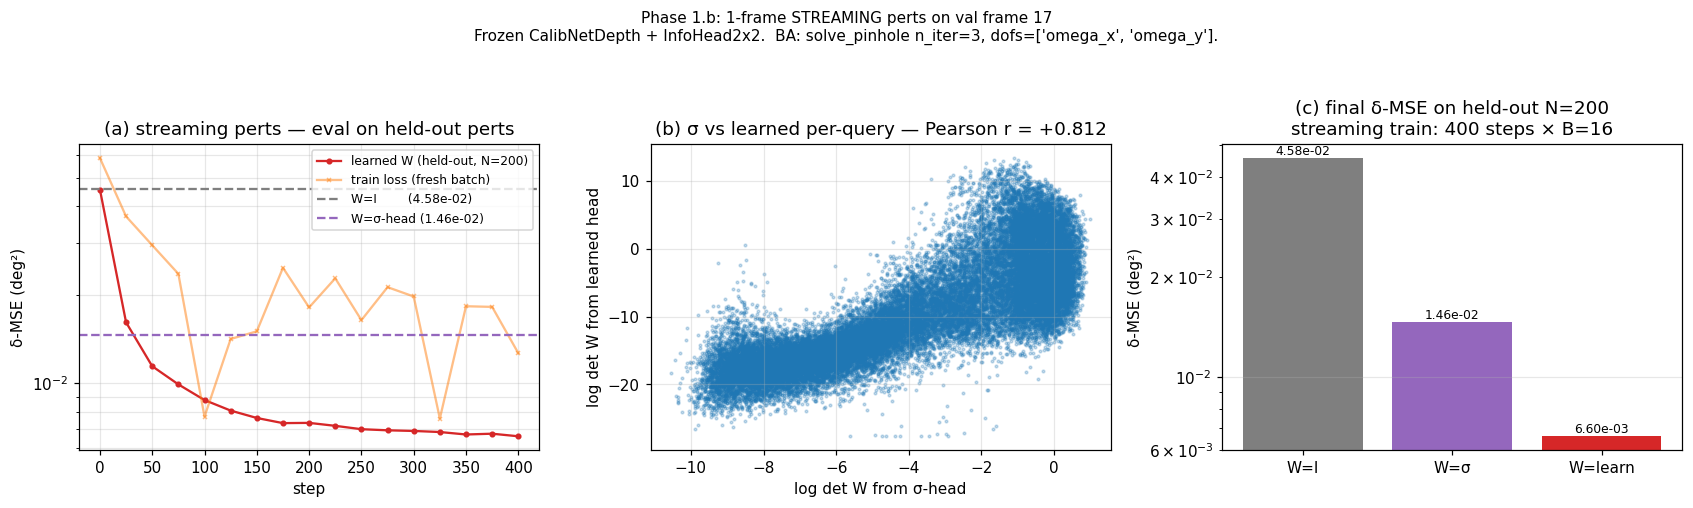
\includegraphics[width=\linewidth]{curves_streaming_idx17.png}
\caption{\textbf{Phase 1.b training curves and head agreement (idx 17).}
\textbf{(a)} Held-out $\delta$-MSE drops from $\sim$$5\times 10^{-2}$
to $6.6\times 10^{-3}$ over 400 steps; horizontal dashed lines mark
$\W{=}I$ and $\W{=}\sigma$-head baselines.
\textbf{(b)} Per-query scatter: each dot is one LiDAR query;
$x$-axis is $\log\det\W$ from the frozen $\sigma$-head, $y$-axis is
$\log\det\W$ from the trained learned head. Pearson $r{=}{+}0.812$.
The two heads agree on most queries (the diagonal cloud of objects:
signs, building edges, vehicles) and disagree on the off-diagonal
band---the road points, where the learned head pushes $\log\det\W$
much lower (much larger ellipses) than the $\sigma$-head.
\textbf{(c)} Final $\delta$-MSE bars on the held-out N=200.}
\label{fig:curves_idx17}
\end{figure}

\subsection{What the heads actually do}

\Cref{fig:hero} (top of paper) shows the two heads as $2{\times}2$
covariance ellipses ($\Sig_i = \W_i^{-1}$) on the anchor tile.
Mean major-axis is $2.6\,$px for the $\sigma$-head versus $57\,$px for
the learned head---a $\sim 22\times$ scale gap concentrated on the
road. Two properties the $\sigma$-head cannot express:

\begin{enumerate}
\item \emph{Suppress the road almost entirely.} Pose is determined by a
  few high-information points, not by averaging a thousand co-planar
  asphalt points.
\item \emph{On the road, distrust the horizontal direction much more
  than the vertical.} Road-plane points slide along the surface; their
  horizontal $\Suv$ is uninformative about yaw. Local residuals look
  isotropic, so the $\sigma$-head has no signal to learn this. The
  learned head develops the anisotropy because horizontal mis-trust is
  what would have improved pose, and the GN gradient penalised it for
  not having that anisotropy.
\end{enumerate}

The scatter in \cref{fig:curves_idx17}(b) makes the same point
quantitatively. The diagonal cloud is the set of queries on which the
$\sigma$-head and the learned head agree (high-information objects).
The off-diagonal band, where the learned head's $\log\det\W$ is far
below the $\sigma$-head's, is the road. NLL-trained $\Sig_\sigma$
calls these points trustworthy because $\Suv$ is locally predictable
there; pose-trained $\W$ calls them the opposite, because trusting
them pulls the GN solution into the ground plane.

\subsection{Degenerate-tile sanity check}

\Cref{tab:combined} also reports the same recipe on val tile 0
(\texttt{00000000\_t0.pt}, asphalt + chain-link fence). On this tile
both $\W{=}I$ and $\W{=}\sigma$-head are \emph{worse than predicting
$\delta{=}0$}: the GN solver actively moves pose into the ground
plane. Only the learned head crosses below the do-nothing line. This
is the introduction's critique in numerical form---per-point NLL is
not a substitute for pose-trust, and uniform weights are not either.

\subsection{Scope of Phase 1.b}

The new head's finetune is confined to a single tile. The frozen
backbone behind it was trained on tens of thousands of frames with
per-point NLL---that is where the pose-relevant signal in the queries
came from. Phase 1.b proves the design assumption: frozen queries
already carry that signal, and an MLP supervised only through the math
layer can recover it. Generalisation \emph{of the new head} across
tiles is Phase 1.c.

% ----- 6.x Phase 1.c ----------------------------------------------------------
\section{Phase 1.c: cross-tile streaming on KAMIKADO}\label{sec:phase1c}

Same recipe, but each training step now draws a fresh
\emph{(training-tile, perturbation)} pair from the KAMIKADO train split
(27\,880 tiles), and the held-out batch is $N{=}512$ random
\emph{validation} tiles, each with one fresh perturbation sampled at
start. The head can no longer overfit to a single scene: the only way
to lower the loss is to learn a function $\mathbf{q} \mapsto \W$ that
generalises across both pose draws and tile content.

\begin{figure}[t]
\centering
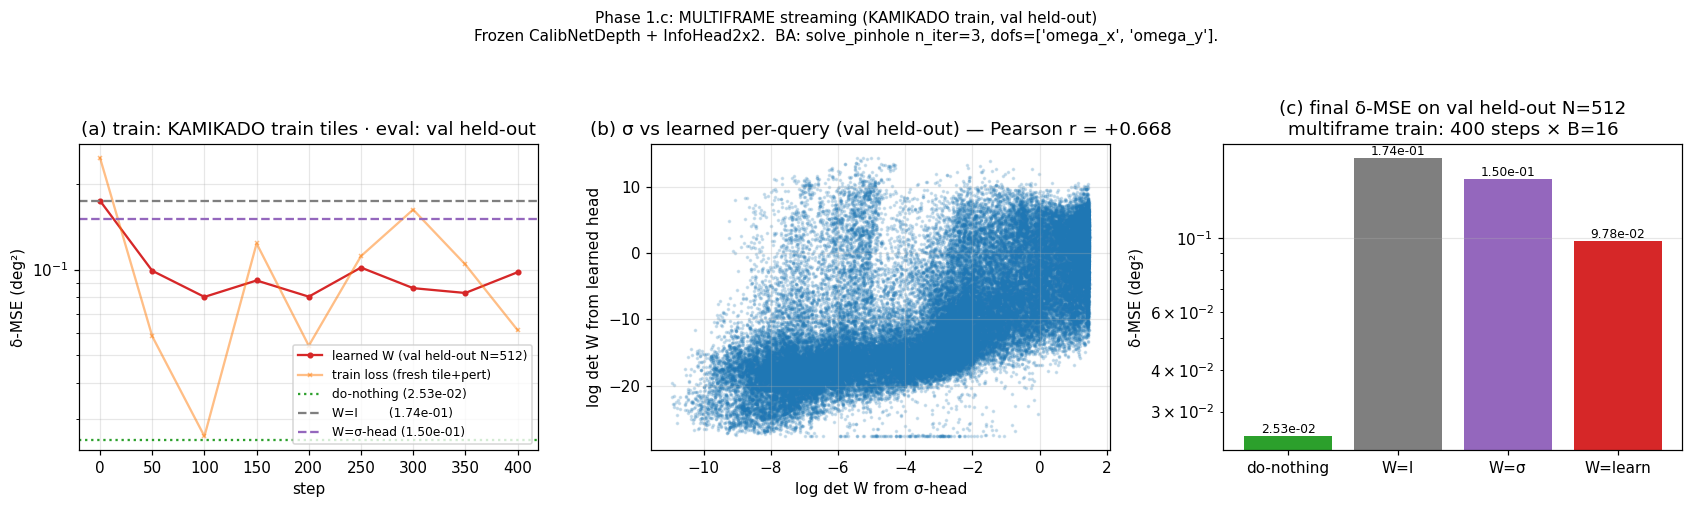
\includegraphics[width=\linewidth]{curves_multiframe.png}
\caption{\textbf{Phase 1.c training curves and head agreement
(KAMIKADO multi-tile).} \textbf{(a)} Held-out $\delta$-MSE drops from
$\sim$$1.7\times 10^{-1}$ (= $\W{=}I$ baseline) to $\sim$$8\times 10^{-2}$
in $\sim$100 steps. Both $\W{=}I$ and the $\sigma$-head sit
\emph{above} the do-nothing line: per-point NLL and uniform weighting
both move pose in the wrong direction across the multi-tile val set.
\textbf{(b)} Per-query scatter (Pearson $r{\sim}{+}0.6$) showing
$\sigma$-head and learned head agree on objects but separate by orders
of magnitude on road-plane queries.
\textbf{(c)} Final $\delta$-MSE bars on val held-out $N{=}512$.}
\label{fig:curves_multiframe}
\end{figure}

\Cref{tab:combined} (Phase 1.c columns) reports the result. The
learned head reaches $\delta$-MSE $0.098\,\mathrm{deg}^2$ versus
$0.150$ for the $\sigma$-head---a $1.5\times$ gain---using the
\emph{exact same architecture and loss} as Phase 1.b but trained
without ever seeing the val tiles. Two structural observations:

\begin{enumerate}
\item \emph{Both $\sigma$-head and $\W{=}I$ are now worse than
do-nothing} ($0.150$ and $0.174$ vs.\ $0.025$). The §1 critique was a
prediction; this is the prediction in numerical form, on the full
KAMIKADO val set rather than one cherry-picked degenerate tile.
\item \emph{The learned head's gap to do-nothing is
$\sim$$4\times$ at this scale} (0.098 vs 0.025). On the single highway
tile of Phase 1.b the gap was reversed by $4.5\times$ in the other
direction. The gap reflects two things the present model cannot fix
without a backbone unfreeze: first, a frozen backbone trained only
with per-point NLL has limited cross-scene capacity in its query
features; second, the head is supervised by $\|\delta-\delta_{gt}\|^2$,
which is invariant to the overall scale of $\W$. The
$\langle\log\det\W\rangle$ of the trained head drifts to $-15$ without
saturating, exactly the symptom of an under-constrained scale.
\end{enumerate}

The second observation directly motivates the next stage: replace the
MSE pose loss with the GN solver's \emph{own} natural likelihood, in
which $\W$ scale is no longer free.

% ----- 7. What's next ---------------------------------------------------------
\section{What's next}\label{sec:next}

\textbf{Phase 1.d: $\delta$-NLL instead of $\delta$-MSE.}
The Gauss--Newton solver returns its own natural covariance for free:
$\Sig_\delta = (\sum_i J_i^\top \W_i J_i)^{-1}$.
Replacing the current MSE pose loss with the corresponding negative
log-likelihood,
%
\begin{equation}
\mathcal{L}_{\delta\text{-NLL}}
\;=\; \tfrac{1}{2}(\delta-\delta_{gt})^\top \Sig_\delta^{-1}
       (\delta-\delta_{gt}) + \tfrac{1}{2}\log\det\Sig_\delta,
\label{eq:dnll}
\end{equation}
%
turns the overall scale of $\W$ from a free parameter into a calibrated
quantity (the second term penalises overconfident pose covariances).
The Phase 1.c symptom of $\langle\log\det\W\rangle\to -15$ without
saturation should disappear, and---more importantly---the per-frame
$\Sig_\delta$ becomes meaningful for the next step.

\textbf{Phase 2 (E2E per-image): one more Gauss--Newton step.}
A KAMIKADO frame is rendered as $\sim 8$ overlapping tiles. The current
phases all report a per-tile $\delta$. Going to per-image is, by
construction, a single extra GN step that we already have all the
ingredients for: each tile already produces $J_i^\top \W_i J_i$ and
$J_i^\top \W_i \Suv_i$, so the per-image solution is just
%
\begin{equation*}
\delta^{\text{image}}
= \Bigl(\sum_t \sum_i J_{t,i}^\top \W_{t,i} J_{t,i}\Bigr)^{-1}
  \sum_t \sum_i J_{t,i}^\top \W_{t,i} \Suv_{t,i},
\end{equation*}
%
i.e.\ accumulate $J^\top \W J$ and $J^\top \W \mathbf{r}$ over all tiles
of a frame and solve once. No new learnable parameters are introduced.
Tiles dominated by featureless ground plane receive low aggregate
information automatically; the per-tile $\mathrm{tr}(J^\top\W J)$
becomes a free diagnostic for ``did this tile contribute to pose''.
Phase 1.d is a hard prerequisite: without a calibrated $\W$ scale, the
per-tile $\Sig_{\delta_t}$ from which the fused $\Sig_{\delta}$ is
built carries no meaning.

\textbf{Stage 4 (joint backbone finetune).} Unfreeze the backbone and
train with $\lambda_{\mathrm{ba}}\!\cdot\!\mathcal{L}_{\delta\text{-NLL}}$
alongside the existing per-point NLL. The Phase 1.b plateau at
$\sim 0.08^\circ$/axis is the half-pixel floor at $128\times 128$
input; the Phase 1.c plateau at $0.31^\circ$/axis is dominated by
cross-scene capacity in the frozen queries. Both are expected to break
under joint unfreezing and/or higher input resolution.

\textbf{Camera augmentation.} Vary $f_x, f_y, k_1\ldots k_4$ per
sample at training time so the network is forced to learn what is
intrinsic (which pixels say ``trust me'') rather than what is
camera-specific.

\textbf{Code.}
\texttt{models/model\_depth.py:InfoHead2x2} (gated by a constructor
flag so old ckpts load unchanged);
\texttt{scripts/\_debug/overfit\_2dof\_ba.py} (Phase 1);
\texttt{scripts/\_debug/overfit\_2dof\_ba\_stream.py} (Phase 1.b);
\texttt{scripts/\_debug/overfit\_2dof\_ba\_multiframe.py} (Phase 1.c);
\texttt{scripts/\_debug/render\_sigma\_ellipse\_compare.py}
(\cref{fig:hero});
\texttt{scripts/training/train\_ps\_v3\_ddp.py --ba-2dof} (Stage 4).

% ----- References -------------------------------------------------------------
\bibliographystyle{IEEEtran}
\begin{thebibliography}{99}
\bibitem{cite:CalibNetDepth}
H.\ Funaya, ``Per-point depth-aware calibration head with NLL
covariance (CalibNetDepth),''
\emph{Internal codebase, e2e\_calib}, 2026.

\bibitem{teed2021droid}
Z.\ Teed and J.\ Deng,
``DROID-SLAM: Deep Visual SLAM for Monocular, Stereo, and RGB-D
Cameras,''
in \emph{NeurIPS}, 2021.

\bibitem{amos2017optnet}
B.\ Amos and J.\ Z.\ Kolter,
``OptNet: Differentiable Optimization as a Layer in Neural Networks,''
in \emph{ICML}, 2017.

\bibitem{gould2021deep}
S.\ Gould et al.,
``Deep Declarative Networks: A New Hope,''
\emph{IEEE TPAMI}, 2021.

\bibitem{brachmann2017dsac}
E.\ Brachmann et al.,
``DSAC --- Differentiable RANSAC for Camera Localization,''
in \emph{CVPR}, 2017.

\bibitem{chen2020bpnp}
B.\ Chen et al.,
``End-to-End Learnable Geometric Vision by Backpropagating PnP
Optimization,''
in \emph{CVPR}, 2020.

\bibitem{kerbl20233dgs}
B.\ Kerbl, G.\ Kopanas, T.\ Leimk\"uhler, and G.\ Drettakis,
``3D Gaussian Splatting for Real-Time Radiance Field Rendering,''
\emph{ACM TOG}, vol.\ 42, no.\ 4, 2023.

\bibitem{iyer2018calibnet}
G.\ Iyer et al.,
``CalibNet: Geometrically Supervised Extrinsic Calibration using 3D
Spatial Transformer Networks,''
in \emph{IROS}, 2018.

\bibitem{schneider2017regnet}
N.\ Schneider et al.,
``RegNet: Multimodal Sensor Registration Using Deep Neural Networks,''
in \emph{IV}, 2017.

\bibitem{lv2021lccnet}
X.\ Lv et al.,
``LCCNet: LiDAR and Camera Self-Calibration using Cost Volume Network,''
in \emph{CVPR Workshops}, 2021.

\bibitem{shi2020netcalib}
J.\ Shi et al.,
``NetCalib: A Novel Approach for LiDAR-Camera Auto-calibration based
on Deep Learning,''
in \emph{ICPR}, 2020.

\end{thebibliography}

\end{document}
